\subsection*{Aufgabe 6}
Die folgende empirische Verteilungsfunktion beschreibt die Verteilung des Merkmals "Alter" in der aktuellen Gesamtheit aller M�tter auf der Entbindungsstation einer gro�en Klinik. \newline \newline
\begin{center}
\begin{figure}[!htbp]
\fbox{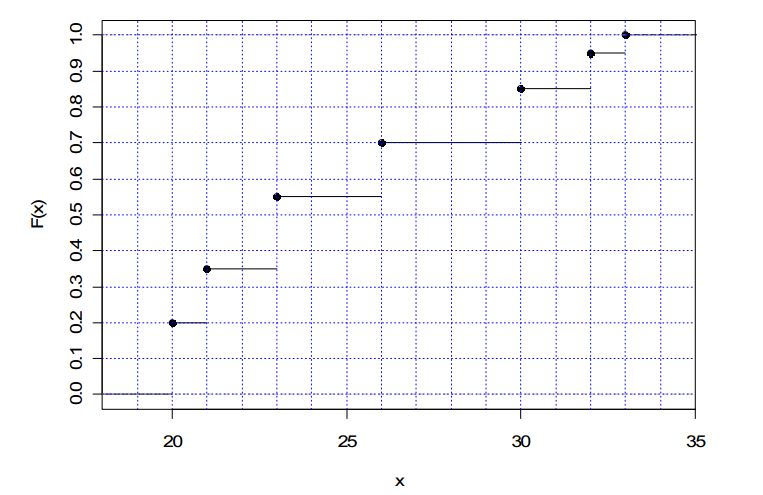
\includegraphics[width=0.9\textwidth,page=1]{./Grafiken/AB_1_6.jpg}} \caption{Erkl�rung}
\end{figure}
\end{center}

\begin{enumerate} [label=\alph*)]
\item Geben Sie die tats�chlich vorkommenden Merkmalsauspr�gungen und die jeweiligen relativen H�ufigkeiten an!
\item Welcher Anteil der M�tter ist �lter als 26 Jahre?
\end{enumerate}


